\documentclass{article}

\usepackage{geometry}
 \geometry{
 a4paper,
 total={170mm,257mm},
 left=20mm,
 top=20mm,
 }

\usepackage[utf8]{inputenc}
\usepackage[russian]{babel}

\usepackage{amsfonts}
\usepackage{amsmath}

\usepackage[none]{hyphenat}

\usepackage{color}

\usepackage{graphicx}
\graphicspath{ {charts/} }

\setlength{\parindent}{0pt}
\setlength{\parskip}{1em}

\begin{document}

{\large

Богдан Уладзіслаў

ФПМІ, 4 курс, 3 група

\vspace{5mm}

Лабараторная работа 1

Крыптааналіз метадаў простай падстаноўкі

}

\vspace{5mm}

\subsection*{1-2. Рэалізацыя праграмнага сродка для шыфравання/дэшыфравання тэкставага файла.}

Праграма рэалізаваная на мове Go.
Працуе з тэкстамі на ангельскай і беларускай мовах (падтрымка іншых моваў
дадаецца праз вызначэнне дадатковых алфавітаў).
Прыклады камандаў, якія ажыццяўляюць шыфраванне/дэшыфраванне:

Шыфраванне тэкста на ангельскай мове (мова па змоўчванні) метадам Цэзара з
выпадкова-згенераваным зрухам:
\begin{verbatim}
  ./lab1-substitutions -encrypt -file=in.txt -out=out.txt
\end{verbatim}

Дэшыфраванне тэкста на беларускай мове, зашыфраванага метадам Цэзара;
ажыццяўляецца з прымяненнем частотнага аналіза:
\begin{verbatim}
  ./lab1-substitutions -decrypt -file=out.txt -out=result.txt -lang=be
\end{verbatim}

Шыфраванне тэкста на ангельскай мове з заданнем ключавога слова (метад Віжэнэра):
\begin{verbatim}
  ./lab1-substitutions -encrypt -file=in.txt -out=out.txt -vigenere_keyword="plot"
\end{verbatim}

Дэшыфраванне тэкста на беларускай мове, зашыфраванага метадам Віжэнэра;
ажыццяўляецца па метадзе Касіскі:
\begin{verbatim}
  ./lab1-substitutions -decrypt -file=out.txt -out=result.txt -lang=be -kasiski_decryption
\end{verbatim}

Зыходны код даступны на GitHub: \url{https://github.com/uladbohdan/uni-code/7-security/lab1-substitutions}

Магчымасці праграмы могуць быць пратэставаныя скрыптом, які знаходзіцца разам з
зыходным кодам (патрэбныя кампілятар go і утыліта diff):
\begin{verbatim}
  bash run_tests.sh
\end{verbatim}

\subsection*{3-4. Эксперыментальнае даследаванне залежнасці імавернасці паспяховага правядзення
атакі па метадзе Касіскі ад даўжыні шыфратэкста і даўжыні ключавога слова.}

\begin{center}
  \begin{tabular}{ | c | c | c | с | c | c | c | }
    \hline
    тэкст / даўжыня ключавога слова & 2 & 3 & 4 & 5 & 6 & 7 \\ \hline
    кароткі ангельскі: 445 сімвалаў & $- (2)$ & $- (6)$ & $- (8)$ & $- (5)$ & $- (6)$ & $- (245)$ \\ \hline
    сярэдні ангельскі: 1686 сімвалаў & + & + & $-$ (1) & $+-$ (5) & $+-$ (6) & $- (1)$ \\ \hline
    доўгі ангельскі: 27103 сімвала & + & + & $- (2)$ & + & $- (2)$ & + \\ \hline
    кароткі беларускі: 559 сімвалаў & $+-$ (4) & + & \minus (8) & $- (10)$ & $- (204)$ & $- (1)$ \\ \hline
    сярэдні беларускі: 1775 сімвалаў & + & + & + & + & + & + \\ \hline
    доўгі беларускі: 61241 сімвал & + & + & $- (2)$ & + & + & + \\
    \hline
  \end{tabular}
\end{center}

Па табліцы:
\begin{enumerate}
  \item $+$ - тэкст цалкам расшыфраваўся, $-$ - тэкст не расшыфраваўся,
  $+-$ - тэкст расшыфраваўся часткова, так, што яго можна чытаць.
  \item у дужках - даўжыня кодавага слова па прадказанні метада Касіскі.
  Часам даўжыня была ўгаданая правільна, але алгарытм не здолеў расшыфраваць
  тэкст праз тое, што кепска спрацаваў частотны аналіз.
  \item вынікі эксперымента дастаткова суб'ектыўныя, вельмі моцна вынік
  залежыць ад падабранага тэкста. Агульная тэндэнцыя, тым не менш, заўважная.
  \item з ростам памера тэкста надзейнасць расце: гэта звязана з тым, што
  правільнасць выканання частотнага аналіза проста залежыць ад памера ўваходных
  дадзеных.
  \item з ростам даўжыні ключавога слова дэшыфраванне працуе горш. Прычыны:
  (а) зашыфраваныя ўчасткі паўтараюцца радзей, адпаведна, складаней высветліць
  даўжыню ключавога слова; (б) неабходнасць выканання частотнага аналіза на
  тэкстах, даўжыня якіх падае з ростам даўжыні ключавога слова.
\end{enumerate}

Візуалізацыя дадзеных з табліцы. Значэнні па восі ардынатаў - адсотак
паспяхова расшыфраванага тэксту.

\begin{center}
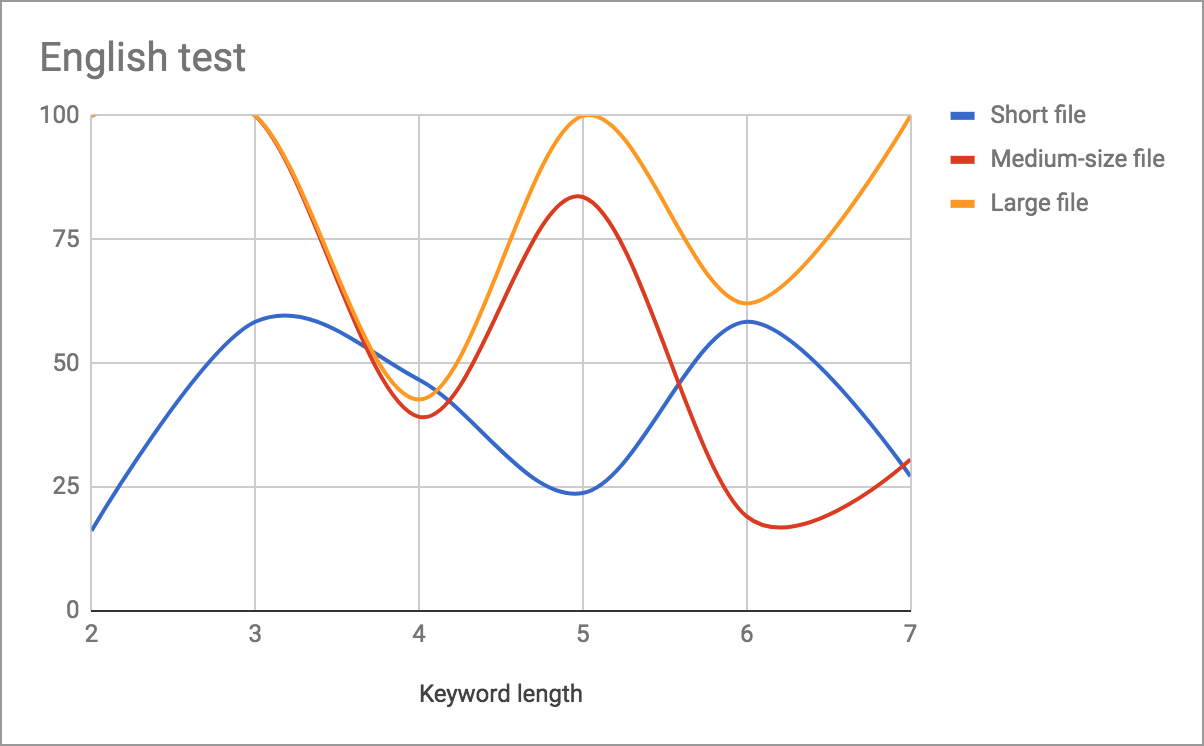
\includegraphics[width=15cm]{en}

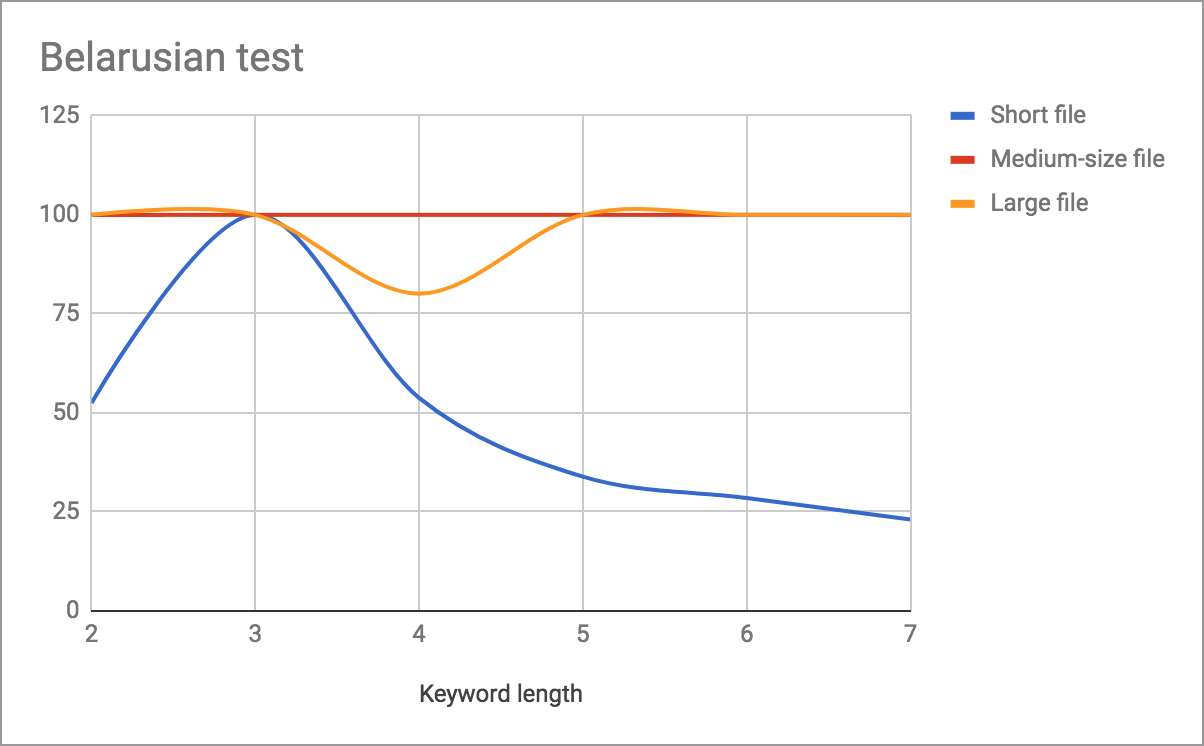
\includegraphics[width=15cm]{be}
\end{center}

\end{document}
